\documentclass[a4paper,twoside,11pt]{article}
\usepackage{a4wide,graphicx,fancyhdr,amsmath,amssymb,float,longtable,chronology,caption,subcaption}
\usepackage{algorithmic}
\usepackage{hyperref}
\usepackage{url}

%----------------------- Macros and Definitions --------------------------

\setlength\headheight{20pt}
\addtolength\topmargin{-10pt}
\addtolength\footskip{20pt}

\newcommand{\N}{\mathbb{N}}
\newcommand{\ch}{\mathcal{CH}}
\everymath{\displaystyle}
\newcommand{\define}[2]{\noindent{\bf #1}}
\newcommand{\scg}{System Validation}

\newcommand{\action}[2]{{\tt #1(#2)}}
\newcommand{\todo}[1]{{\color{red}#1}}

\fancypagestyle{plain}{%
	\fancyhf{}
	\fancyhead[LO,RE]{\sffamily\bfseries\large Technische Universiteit Eindhoven}
	\fancyhead[RO,LE]{\sffamily\bfseries\large 2IMF30 \scg}
	\fancyfoot[LO,RE]{\sffamily\bfseries\large Department of Mathematics and Computer Science}
	\fancyfoot[RO,LE]{\sffamily\bfseries\thepage}
	\renewcommand{\headrulewidth}{0pt}
	\renewcommand{\footrulewidth}{0pt}
}

\pagestyle{fancy}
\fancyhf{}
\fancyhead[RO,LE]{\sffamily\bfseries\large Technische Universiteit Eindhoven}
\fancyhead[LO,RE]{\sffamily\bfseries\large 2IMF30 - System Validation}
\fancyfoot[LO,RE]{\sffamily\bfseries\large Department of Mathematics and Computer Science}
\fancyfoot[RO,LE]{\sffamily\bfseries\thepage}
\renewcommand{\headrulewidth}{1pt}
\renewcommand{\footrulewidth}{0pt}

%-------------------------------- Title ----------------------------------

\title{\sffamily\bfseries 2IMF30 \scg\ - Project 1}
\author{Tom van Diggelen \qquad Student number: 0745801 \\{\tt t.w.t.v.diggelen@student.tue.nl}\\ \\ Huib Donkers \qquad Student number: 0769015 \\{\tt h.t.donkers@student.tue.nl} \\ \\ Jeroen Noten \qquad Student number: 0784113 \\{\tt j.f.h.noten@student.tue.nl}\\ \\ Mart Pluijmaekers \qquad Student number: 0753117 \\{\tt m.h.l.pluijmaekers@student.tue.nl} \\ \\ Hein van Beers \qquad Student number: 0765658 \\{\tt h.a.v.beers@student.tue.nl}}

\date{\today}

%--------------------------------- Text ----------------------------------

\begin{document}
\maketitle
\tableofcontents

\begin{figure}[h]
    \centering
	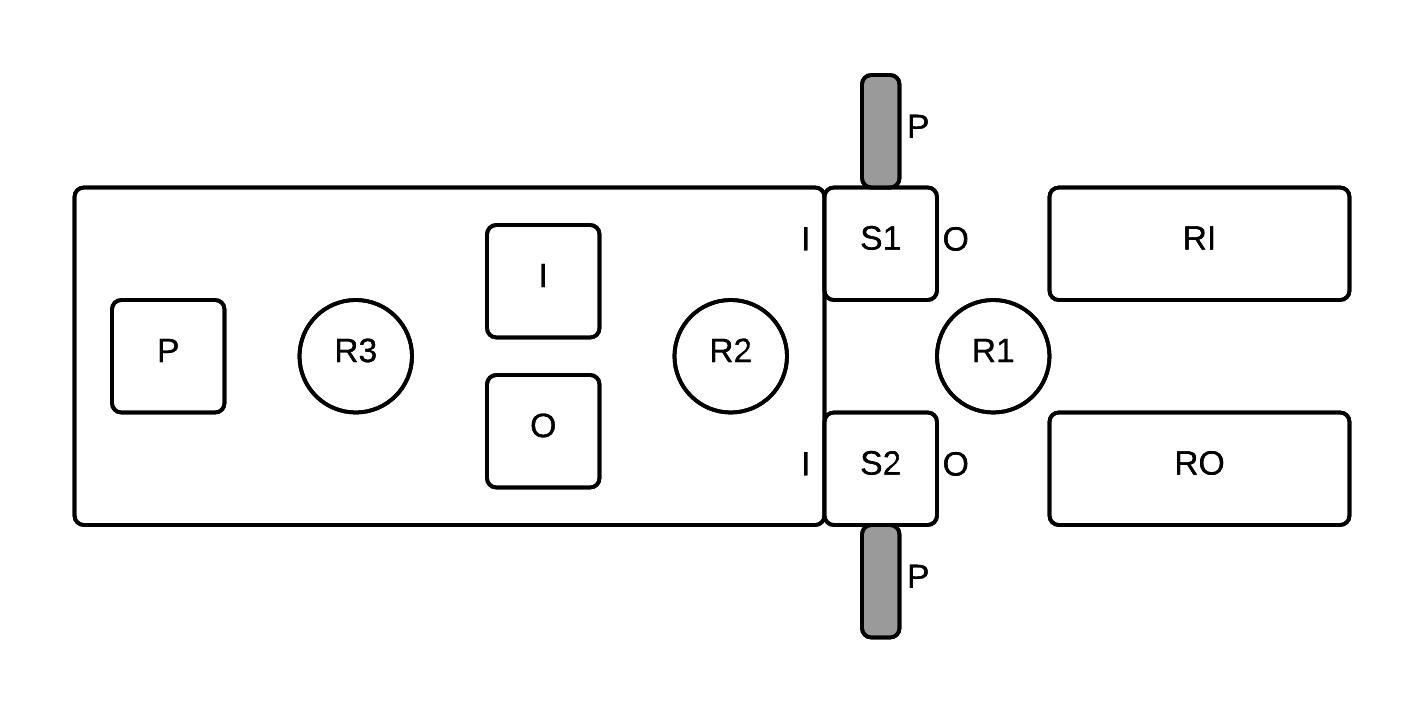
\includegraphics[width=0.7\textwidth]{waferstepper.png}
\end{figure}

\newpage
\section{Introduction}

\section{Basic requirements}
% !TEX root = ../report.tex
\subsection{Definitions}
\begin{enumerate}
  \item A wafer is considered processed when the projector has finished processing and the wafer has exited the stepper.
\end{enumerate}

\subsection{Assumptions}
\begin{enumerate}
  \item The doors are the only part of the machines that can malfunction.
  \item The main room is assumed to always be a vacuum.
  \item The external input and output racks are assumed to be infinite in size.
  \item Sluice pumps change the air pressure to either zero or one atmosphere.
\end{enumerate}

\subsection{Requirements}
\begin{enumerate}
  \item At least one door of a sluice is closed at any point in time.
  \item No robot may interact with a sluice whenever its access door is closed.
  \item An unprocessed wafer will eventually be processed.
  \item Internal racks, sluices, and the projector place each contain at most one wafer.
  \item When the projector is at work, no interaction with the wafer is permissible.
  \item A sluice door cannot open until the pressure on both sides is equal.
  \item Sluice pumps will not operate until both of its doors are closed.
  \item \todo{Restricties voor robots toevoegen}
\end{enumerate}


\section{Actions}
\begin{tabular}{|l|l|l|p{4cm}|}
\hline  
  \textbf{Action} & \todo{\textbf{Executed by}} & \textbf{Variables} & \textbf{Meaning} \\
  \hline
  \todo{\action{get}{$p$}} & Robots & $p$: A place in the system & Get a wafer from place $p$\\
  \hline
  \todo{\action{put}{$p$}} & Robots & $p$: A place in the system & Put a wafer on place $p$\\
  \hline
  \action{project}{} & Projector & None & Project a wafer\\
  \hline
  \action{openInside}{$s$} & Inside sluice doors & $s$: The corresponding sluice & Open the inside sluice door of sluice $s$\\
  \hline
  \action{openOutside}{$s$} & Outside sluice doors & $s$: The corresponding sluice & Open the outside sluice door of sluice $s$\\
  \hline
  \action{closeInside}{$s$} & Inside sluice doors & $s$: The corresponding sluice & Close the inside sluice door of sluice $s$\\
  \hline
  \action{closeOutside}{$s$} & Outside sluice doors & $s$: The corresponding sluice & Close the outside sluice door of sluice $s$\\
  \hline
  \action{Vacuum}{$s$} & Pumps & $s$: The corresponding sluice & Make sluice $s$ into a vacuum\\
  \hline
  \action{deVacuum}{$s$} & Pumps & $s$: The corresponding sluice & Make sluice $s$ into normal air pressure\\
  \hline
  \action{read}{$s$} & Sensors & $s$: The corresponding sluice & Read the value of the sensor in sluice $s$\\
  \hline
\end{tabular}

\section{Requirements in terms of actions}
% !TEX root = ../report.tex

Expressing every requirement in terms of actions.

\begin{description}
 \item[At least one door of a sluice is closed at any point in time] \hfill \\
 For any sluice $s$:
 \begin{itemize}
  \item Between any \action{openInside}{$s$} and its most recent preceding \action{closeOutside}{$s$}, there may not be an \action{openOutside}{$s$}
  \item Between any \action{openOutside}{$s$} and most its recent preceding \action{closeInside}{$s$}, there may not be an \action{openInside}{$s$}
 \end{itemize}

 \item[No robot may interact with a sluice whenever its access door is closed] \hfill \\
 \todo{put/move/get definitie final maken}
 
 \item[An unprocessed wafer will eventually be processed] \hfill \\
 \todo{Kan niet echt (makkenlijk) in traces uitgedrukt worden...}
 
 \item[Internal racks, sluices and the projector each contain one wafer] \hfill \\
 \todo{put/move/get definitie final maken}
 
 ``Voordat een robot iets op internal rack/sluice of projector kan leggen, moet de vorige zin weggehaald.''
 
 \item[When the projector is at work, no interaction with the water is permissible] \hfill \\
 \todo{put/move/get definitie final maken}
 
 \todo{\'of haal de requirement weg, \' of gebruik \action{beginProjection}{} en \action{endProjection}{} actions}
 
 \todo{dubbele requirement?}
 
 \item[Sluice pumps change the air pressure to either zero or one atmosphere.] \hfill \\
 \todo{Tja... volgens mij een assumption, geen requirement. Dit valt niet in traces uit te drukken}
 
 \item[A sluice door cannot open untill the pressure on both sides is equal] \hfill \\
 For any sluice $s$:
 \begin{enumerate}
  \item Between any \action{openInside}{$s$} and its most recent preceding \action{Vacuum}{$s$}, there may not be a \action{deVacuum}{$s$}
  \item Between any \action{openOutside}{$s$} and its most recent preceding \action{deVacuum}{$s$}, there may not be a \action{Vacuum}{$s$}
 \end{enumerate}

 \item[Sluice pumps cannot operate until both of its doors are closed] \hfill \\
 For any sluice $s$:
 \begin{enumerate}
  \item Between any \action{Vacuum}{$s$} or \action{deVacuum}{$s$} and its most recent preceding \action{closeInside}{$s$}, there may not be a \action{openInside}{$s$}
  \item Between any \action{Vacuum}{$s$} or \action{deVacuum}{$s$} and its most recent preceding \action{closeOutside}{$s$}, there may not be a \action{openOutside}{$s$}
 \end{enumerate}

 \item[$R3$ will not take a wafer from $I$ when $P$ is occupied] \hfill \\
 \todo{put/move/get definitie final maken}
 
 \item[$R3$ will not put wafers in $I$] \hfill \\
 \todo{put/move/get definitie final maken}
 
 \item[$R3$ will not take wafers from $O$] \hfill \\
 \todo{put/move/get definitie final maken}
 
 \item[$R3$ will not take a wafer from $P$ when the projector is at work] \hfill \\
 \todo{put/move/get definitie final maken}
 
 \todo{\'of haal de requirement weg, \' of gebruik \action{beginProjection}{} en \action{endProjection}{} actions}
 
 \todo{dubbele requirement?}
 
\end{description}


\begin{thebibliography}{9}

\end{thebibliography}


\end{document}
